\documentclass[pdf,hyperref={unicode}, aspectratio=43, serif,11pt]{beamer}
\usepackage[T2A]{fontenc}
\usepackage[english, russian]{babel}  

%Задаем параметры документа
% \usepackage[top = 20 mm, 
%             bottom = 20 mm, 
%             left = 30 mm, 
%             right = 30 mm]{geometry}
            
%Красная строка в первом абзаце
\usepackage{indentfirst}
%Величина отступа красной строки
\setlength{\parindent}{12.5 mm}

%Межстрочный интервал
%\def\baselinestretch{1.5}
\usepackage{setspace}
\setstretch{1}

\title[ФизМат]{Физико-математический факультет}
\author{М.В. Зенкин}
\date{5 мая 2022}
\institute[]{Орловский государственный
университет имени И.\,С.~Тургенева}
\def\baselinestretch{1}

\usefonttheme[onlymath]{serif}
\usepackage{beamerthemesplit}

%тема оформления
\usetheme{Madrid}%Warsaw

%цветовая гамма
\usecolortheme{seahorse}%whale


\begin{document}
\begin{frame}
\titlepage
\end{frame}


\begin{frame}
\frametitle{История факультета}
\tiny{Пятого августа 1931 года СНК РСФСР распорядился создать в Орле индустриально-педагогический институт. 16 октября первые студенты, 121 человек, и 11 преподавателей приступили к занятиям на четырех факультетах: физико-техническом, химическом, социально-экономическом и политехническом. Под студенческое общежитие было отведено здание на улице Садовой, 29 (ныне ул. Горького).

Первые преподаватели физико-технического факультета – это: Болдырев – директор института, читал историю ВКП(б) и Коминтерна, А.Д. Скопин – заместитель директора по учебной работе, вел военное дело, А.И. Шмаков – доцент, заведующий кафедрой педагогики, преподавал педагогику и психологию, Грушинский – преподаватель физкультуры, В.А. Александров – математик, Воскресенский – физик, Бондарева – математик, Яськов – черчение.

В 1932 году индустриально-педагогический институт преобразован в педагогический, физико-технический факультет – в физико-математический. В этом же году открыты рабфак и вечернее отделение с двумя факультетами: физико-математическим и литературным. Открыто заочное отделение с теми же факультетами, что и на стационаре.}
\begin{figure}[!h]
\centering
\center{\includegraphics[scale=0.2]{1.jpg}\\
Рис. 1 - Первые преподаватели}
\end{figure}

\end{frame}

\begin{frame}
\frametitle{Факультет в годы Великой Отечественной войны}
\tiny{
В годы Великой Отечественной войны 24 преподавателя и студента Дмитрий Сорин пали в боях за Родину. В их числе преподаватель М.А. Александров, декан физмата П.Д. Ерёмин, заведующий кафедрой педагогики В.Ф. Недешев, секретарь комитета комсомола института Н.А. Прудников, студент физмата Герой Советского Союза В.А. Булычев, студент физмата подпольщик Дмитрий Сорин (расстрелян фашистами в 1942 году) посмертно награжден медалью «За отвагу».

В послевоенные годы кафедрой математического анализа заведовал доцент Сергей Митрофанович Клименко. Он же являлся деканом до 1947 года, кафедрой физики – Сергей Дмитриевич Токарев, кафедрой алгебры и геометрии – исполняющий обязанности доцента Б.И. Аргунов.

Особенностью учебного процесса в послевоенный период стало то, что часть студентов пришла на факультет с фронта – завершить начатое в 30-х обучение, либо поступить на 1 курс. Учились такие парни, как правило, на «отлично». Среди них были Копаев Владимир Антонович, Парнасский Иван Васильевич. Сталинскими стипендиатами в 1947–49 годы были Иножарский Вениамин Константинович и Ростовцев Николай Михайлович. После выпуска они работали преподавателями физико-математического факультета. Алексеев Алексей Петрович окончил физмат в 1948 году, в 1953 году возглавил его как декан.
.}
\begin{figure}[!h]
\centering
\center{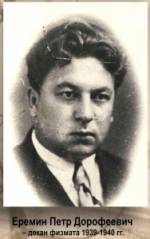
\includegraphics[scale=0.5]{2.1.jpg}
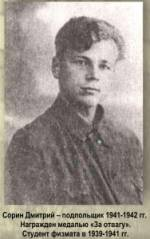
\includegraphics[scale=0.5]{2.2.jpg}\\
Рис. 2 - Преподаватели/студенты в годы Великой Отечественной войны}
\end{figure}

\end{frame}
\begin{frame}
\frametitle{Послевоенное время}
\tiny{
В 1957 году 30 июля было сдано в эксплуатацию новое здание педагогического института на улице Комсомольская, 95. Физико-математический факультет занял 4-й этаж. До сегодняшнего дня факультет адреса не изменил.Во второй половине 1980-х годов наращивался темп компьютеризации учебного процесса на факультете. Так, в 1989 году физмат получил 10 новых компьютеров марки IBM. На факультете их стало 18. Была оборудована компьютерная аудитория на первом этаже – 132-я.

Основным событием первой половины 1990-х годов стало преобразование Орловского государственного педагогического института в Орловский государственный педагогический университет (1994 г.).В 1996 году Орловский государственный педагогический университет преобразован в Орловский государственный университет.

.}
\begin{figure}[!h]
\centering
\center{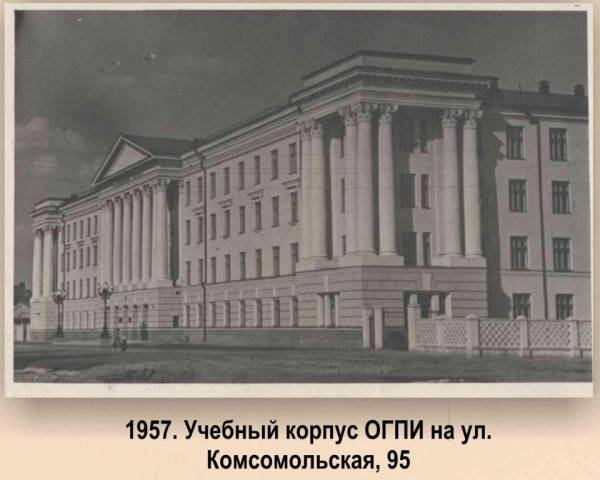
\includegraphics[scale=0.3]{3.jpg}\\
Рис. 3 - Здание педагогического института}
\end{figure}

\end{frame}
\begin{frame}
\frametitle{Деканы факультета}

\begin{table}[h]\begin{center}
\scalebox{0.6}{

\begin{tabular}{|c|c|}

\hline
{ 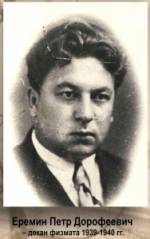
\includegraphics[scale=0.4]{2.1.jpg}} & 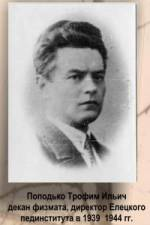
\includegraphics[scale=0.4]{pol.jpg} \\ \hline
\multicolumn{1}{|c|}{1940 - 1941 Еремин Петр Дорофеевич} & \begin{tabular}[c]{@{}c@{}}1934 - 1938 Поледько Трофим Ильич\end{tabular} \\ \hline
{ 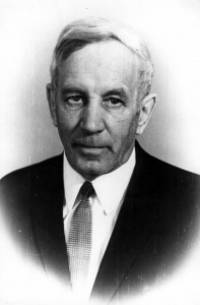
\includegraphics[scale=0.4]{gor.jpg}} & { 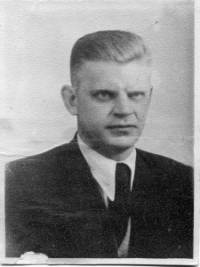
\includegraphics[scale=0.4]{alex.jpg}} \\ \hline
1948 - 1953 Горшенин Святослав Михайлович & \begin{tabular}[c]{@{}c@{}}1953 - 1957 Алексеев Алексей Петрович\end{tabular} \\ \hline
{ 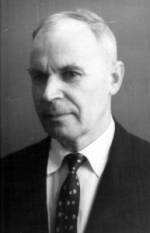
\includegraphics[scale=0.4]{klim.jpg}} & { 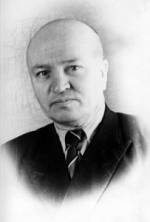
\includegraphics[scale=0.4]{alexand.jpg}} \\ \hline
1941 - 1947 Клименко Сергей Викторович & \begin{tabular}[c]{@{}c@{}}1957 - 1984 Александров Василий Александрович\end{tabular} \\ \hline

\end{tabular}}
\end{center}
\end{table}

\end{frame}

\begin{frame}
\frametitle{В настоящее время}
\tiny{

На факультете функционирует 7 кафедр: математического анализа и дифференциальных уравнений (заведующий – доктор физико-математических наук, профессор А.Н. Зарубин); алгебры и математических методов в экономике (заведующий – доктор педагогических наук, профессор В.Д. Селютин); геометрии и методики преподавания математики (заведующий – доктор педагогических наук, профессор О.В. Тарасова); информатики (заведующий – кандидат физико-математических наук, доцент В.И. Дорофеева); экспериментальной и теоретической физики (заведующий – доктор физико-математических наук, профессор О.И. Марков); высшей математики (заведующий – доктор технических наук, профессор В.А. Гордон); математики и прикладных информационных технологий (заведующий – доктор педагогических наук, профессор Ф.С. Авдеев).

Обучение студентов осуществляется по следующим направлениям бакалавриата и магистратуры: 01.03.01, 01.04.01 Математика, 01.03.02, 01.04.02 Прикладная математика и информатика, 03.03.02, 03.04.02 Физика, 44.03.05, 44.04.01 Педагогическое образование, 09.03.03, 09.04.03 Прикладная информатика.

Выпускники факультета востребованы на рынке труда и находят себе работу в самых разных организациях и учреждениях.
.}
\begin{figure}[!h]
\centering
\center{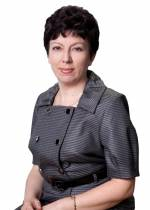
\includegraphics[scale=0.4]{4.jpg}\\
Рис. 4 - Декан факультета, кандидат физико-математических наук, профессор Т.Н. Можарова}
\end{figure}

\end{frame}


\end{document}




\fontsize{14}{18}\selectfont
\thispagestyle{empty}
\newpage
\tableofcontents
\newpage

\section{Набор формул}

\begin{center}
{\bf Степени и индексы}
\end{center}

\noindent $\blacktriangleright$ Набор в \LaTeX:
\begin{lstlisting}
$$
R_{i,j}^{k,n}
$$
\end{lstlisting}

\noindent $\blacktriangleright$ На печати 
$$
R_{i,j}^{k,n}
$$

\begin{center}
{\bf Дроби}    
\end{center}

\noindent $\blacktriangleright$ Набор в \LaTeX:
\begin{lstlisting}
$$
\frac{1}{2}, 
\frac{1}{1+\frac{1}{2}}
$$
\end{lstlisting}
\noindent $\blacktriangleright$ На печати 
$$
\frac{1}{2}, \frac{1}{1+\frac{1}{2}}
$$

\noindent $\blacktriangleright$ Набор в \LaTeX:
\begin{lstlisting}
$$
\dfrac{1}{2}, 
\dfrac{1}{1+\dfrac{1}{2}}
$$
\end{lstlisting}
\noindent $\blacktriangleright$ На печати 
$$
\dfrac{1}{2}, \dfrac{1}{1+\dfrac{1}{2}}
$$

\begin{center}
{\bf Скобки переменного размера}    
\end{center}

\noindent $\blacktriangleright$ Набор в \LaTeX:
\begin{lstlisting}
$$
\left.
\left(T
\right) \dfrac{1}{2}
\right)
$$
\end{lstlisting}

$$
\left.
\left(T
\right) \dfrac{1}{2}
\right)
$$



Корни
$$
\sqrt{4}
$$

Штрифи и многоточия
$$
f''
$$
$$
\ldots \cdots \vdots \ddots 
$$

Имена математических функций
$$
\sin() \cos() \tanh \log_{10}{2} \ln
$$
Греческий алфавит
$$\alpha, \beta \Sigma \sigma \epsilon \varepsilon$$
Символы
$$
\diamond
\blacktriangleleft
$$

Операции с пределами и без
$$
\left.\int\limits_{-\infty}^{+\infty} \sin() \, dx = -\cos(x)\right|_{a}^{b}
$$
$$
\sum\limits_{i=1}^{n}
$$

Нумерация формул
\begin{equation} \label{eq2}
\cos(x)    
\end{equation}

\begin{verbatim}
\begin{equation*} 
\sin(x)    \leqno{(**)}
\end{equation*}
\end{verbatim}


\begin{equation*} 
\sin(x) \leqno{(**)}
\end{equation*}

\begin{equation*} 
\cos(x)  \eqno{(12)}  
\end{equation*}

Включение текста в формулы \eqref{eq2}

\begin{center}
Надстрочные символы
\end{center}
$$
\overline{1,k}, \quad
\hat{x} \quad
\widehat{AB} \quad
\overrightarrow{AB}
$$
Для набора матриц используются следующие окружения:
$$
\begin{pmatrix}
a_{11} & a_{12} & \ldots & a_{1n}\\
a_{21} & a_{22} & \ldots & a_{2n}\\
\vdots & \vdots & \ddots & \vdots \\
a_{n1} & a_{n2} & \ldots & a_{nn}
\end{pmatrix}
$$

$$
\begin{vmatrix}
a_{11} & a_{12} & \ldots & a_{1n}\\
a_{21} & a_{22} & \ldots & a_{2n}\\
\vdots & \vdots & \ddots & \vdots \\
a_{n1} & a_{n2} & \ldots & a_{nn}
\end{vmatrix}
$$

\begin{equation*} 
\sin(x)    \leqno{(**)}
\end{equation*}

$$
\left(
\begin{array}{cccc}
a_{11} & a_{12} & \ldots & a_{1n}\\
a_{21} & a_{22} & \ldots & a_{2n}\\
\vdots & \vdots & \ddots & \vdots \\
a_{n1} & a_{n2} & \ldots & a_{nn}
\end{array}
\right)
$$
\parbox{75 mm}{\begin{multline} 
1+2+3+4+5+ \\
+6+7+8+ \\
 +9+10 = 45. 
\end{multline}}
\parbox{75 mm}{\begin{multline} 
1+2+3+4+5+ \\
+6+7+8+ \\
 +9+10 = 45. 
\end{multline}}

Многострочные выключные формулы

\begin{multline*} 
1+2+3+4+5+ \\
+6+7+8+ \\
 +9+10 = 45. 
\end{multline*}

\begin{gather} %\notag
1+2=3, \notag \\
1+4=5, \\
100+101 = 201.
\end{gather}

\begin{align}  %\notag
1+2=3, \\
1+4=5, \notag \\
100+101 = 201.
\end{align}


\begin{equation}
\begin{split}
1999&=1000+900+{}\\
&+90+9
\end{split}
\end{equation}

\begin{align}
7\times 9& =63 & 63:9& =7\\
9\times 10& =90 & 90:10& =9
\end{align}


Пробелы в формулах вручную \\
\begin{tabular}{|c|c|c|}
\hline
Синтаксис в \LaTeX & Комментарий & Примеры \\ \hline
\begin{lstlisting}
$x\quad y$
\end{lstlisting}
& Пробел в 1em
& $x\quad y$ \\ \hline
\begin{lstlisting}
$x\qquad y$
\end{lstlisting}
& Пробел в 2em
& $x\qquad y$ \\ \hline
\begin{lstlisting}
$\int\sin(x)dx$
\end{lstlisting}
& Без пробела
& $\int\sin(x)dx$\\ \hline
\begin{lstlisting}
$\int\sin(x)\!dx$
\end{lstlisting}
& Отрицательный пробел
& $\int\sin(x)\!dx$\\ \hline
\begin{lstlisting}
$\int\sin(x)\,dx$
\end{lstlisting}
& Тонкий пробел
& $\int\sin(x)\,dx$\\ \hline
\begin{lstlisting}
$\int\sin(x)\:dx$
\end{lstlisting}
& Средний пробел
& $\int\sin(x)\:dx$\\ \hline
\begin{lstlisting}
$\int\sin(x)\;dx$
\end{lstlisting}
& Толстый пробел
& $\int\sin(x)\;dx$\\ \hline
\end{tabular}

Листинги

\begin{lstlisting}
\begin{equation}
\begin{split}
1999&=1000+900+{}\\
&+90+9
\end{split}
\end{equation}
\end{lstlisting}

\section{Набор текста}

\section{Верстка таблиц}

\section{Подготовка презентаций}

\end{document}

